\begin{figure}[ht]
\centering
\resizebox{\textwidth}{!}{
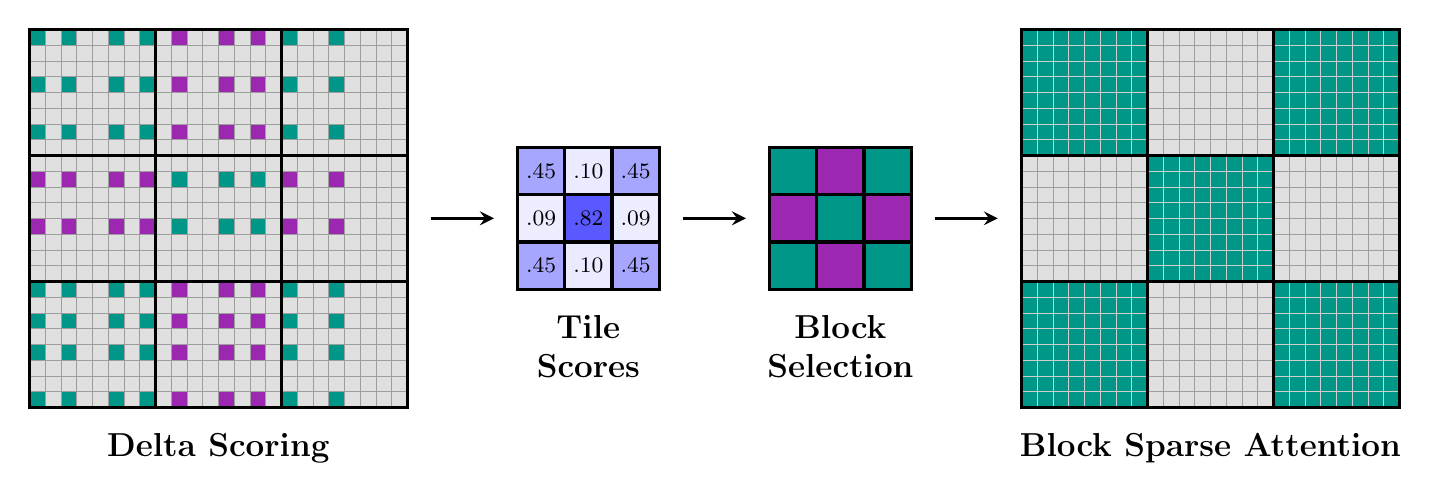
\begin{tikzpicture}[>=stealth, thick]

  % Colors
  \definecolor{selcolor}{HTML}{009688} % Teal
  \definecolor{unselcolor}{HTML}{9C27B0} % Purple
  \definecolor{bglight}{HTML}{E0E0E0}
  \definecolor{gridcolor}{HTML}{9E9E9E}

  \def\cell{0.2} % cell size for left and right
  \def\bcell{1.6} % big cell size = 8 * 0.2
  \def\mcell{0.6} % small (3x3) grid cell size

  % PART 1: Delta Scoring
  \begin{scope}[shift={(0,0)}]
    % Draw background and small grid
    \fill[bglight] (0,0) rectangle (3*\bcell, -3*\bcell);
    \draw[gridcolor, very thin, step=\cell] (0,0) grid (3*\bcell, -3*\bcell);

    % Draw grid-sampled cells: intersection of Q-anchor rows and K-anchor cols
    \foreach \br in {0,1,2} {
      \foreach \bc in {0,1,2} {
        % Determine if block is selected: X pattern => br == bc or br+bc == 2
        \pgfmathtruncatemacro{\issel}{(\br==\bc) || (\br+\bc==2)}
        \ifnum\issel=1
          \colorlet{dcolor}{selcolor}
        \else
          \colorlet{dcolor}{unselcolor}
        \fi

        \foreach \r in {0,...,7} {
          \foreach \c in {0,...,7} {
            % Q anchors depend on the block-row, K anchors on the block-column,
            % so each tile gets its own content-adaptive grid.
            \pgfmathtruncatemacro{\isrow}{
              ((\br==0) && ((\r==0)||(\r==3)||(\r==6))) ||
              ((\br==1) && ((\r==1)||(\r==4))) ||
              ((\br==2) && ((\r==0)||(\r==2)||(\r==4)||(\r==7)))
            }
            \pgfmathtruncatemacro{\iscol}{
              ((\bc==0) && ((\c==0)||(\c==2)||(\c==5)||(\c==7))) ||
              ((\bc==1) && ((\c==1)||(\c==4)||(\c==6))) ||
              ((\bc==2) && ((\c==0)||(\c==3)))
            }
            \pgfmathtruncatemacro{\isgrid}{\isrow && \iscol}
            \ifnum\isgrid=1
              \fill[dcolor] ({\bc*\bcell + \c*\cell}, {-\br*\bcell - \r*\cell}) rectangle ++(\cell, -\cell);
              \draw[gridcolor, very thin] ({\bc*\bcell + \c*\cell}, {-\br*\bcell - \r*\cell}) rectangle ++(\cell, -\cell);
            \fi
          }
        }
      }
    }
    % Draw thick big block borders
    \draw[very thick, step=\bcell] (0,0) grid (3*\bcell, -3*\bcell);
    \draw[very thick] (0,0) rectangle (3*\bcell, -3*\bcell);
    \node[below, font=\large\bfseries] at (1.5*\bcell, -3*\bcell - 0.2) {Delta Scoring};
  \end{scope}

  % Arrow 1
  \draw[->, very thick] (3*\bcell + 0.3, -1.5*\bcell) -- ++(0.8, 0);

  % PART 2: Tile Scores (weight per tile, normalized per query row)
  \begin{scope}[shift={(3*\bcell + 1.4, -1.5*\bcell + 1.5*\mcell)}]
    \foreach \br/\bc/\val/\xf in {
      0/0/.45/35, 0/1/.10/8,  0/2/.45/35,
      1/0/.09/7,  1/1/.82/65, 1/2/.09/7,
      2/0/.45/35, 2/1/.10/8,  2/2/.45/35}
    {
      \fill[blue!\xf] (\bc*\mcell, -\br*\mcell) rectangle ++(\mcell, -\mcell);
      \draw[very thick] (\bc*\mcell, -\br*\mcell) rectangle ++(\mcell, -\mcell);
      \node[font=\footnotesize] at ({(\bc+0.5)*\mcell}, {-(\br+0.5)*\mcell}) {\val};
    }
    \draw[very thick] (0,0) rectangle (3*\mcell, -3*\mcell);
    \node[below, align=center, font=\large\bfseries] at (1.5*\mcell, -3*\mcell - 0.2) {Tile\\Scores};
  \end{scope}

  % Arrow 2
  \draw[->, very thick] (3*\bcell + 1.4 + 3*\mcell + 0.3, -1.5*\bcell) -- ++(0.8, 0);

  % PART 3: Block Selection
  \begin{scope}[shift={(3*\bcell + 1.4 + 3*\mcell + 1.4, -1.5*\bcell + 1.5*\mcell)}]
    \foreach \br in {0,1,2} {
      \foreach \bc in {0,1,2} {
        \pgfmathtruncatemacro{\issel}{(\br==\bc) || (\br+\bc==2)}
        \ifnum\issel=1
          \fill[selcolor] (\bc*\mcell, -\br*\mcell) rectangle ++(\mcell, -\mcell);
        \else
          \fill[unselcolor] (\bc*\mcell, -\br*\mcell) rectangle ++(\mcell, -\mcell);
        \fi
        \draw[very thick] (\bc*\mcell, -\br*\mcell) rectangle ++(\mcell, -\mcell);
      }
    }
    \draw[very thick] (0,0) rectangle (3*\mcell, -3*\mcell);
    \node[below, align=center, font=\large\bfseries] at (1.5*\mcell, -3*\mcell - 0.2) {Block\\Selection};
  \end{scope}

  % Arrow 3
  \draw[->, very thick] (3*\bcell + 1.4 + 3*\mcell + 1.4 + 3*\mcell + 0.3, -1.5*\bcell) -- ++(0.8, 0);

  % PART 4: Block Sparse Attention
  \begin{scope}[shift={(3*\bcell + 1.4 + 3*\mcell + 1.4 + 3*\mcell + 1.4, 0)}]
    \fill[bglight] (0,0) rectangle (3*\bcell, -3*\bcell);
    \draw[gridcolor, very thin, step=\cell] (0,0) grid (3*\bcell, -3*\bcell);

    \foreach \br in {0,1,2} {
      \foreach \bc in {0,1,2} {
        \pgfmathtruncatemacro{\issel}{(\br==\bc) || (\br+\bc==2)}
        \ifnum\issel=1
          \fill[selcolor] (\bc*\bcell, -\br*\bcell) rectangle ++(\bcell, -\bcell);
          % We can re-draw the small grid over it if we want it to look like the original
          \draw[gridcolor!50!white, very thin, step=\cell, shift={(\bc*\bcell, -\br*\bcell)}] (0,0) grid (\bcell, -\bcell);
        \fi
      }
    }

    \draw[very thick, step=\bcell] (0,0) grid (3*\bcell, -3*\bcell);
    \draw[very thick] (0,0) rectangle (3*\bcell, -3*\bcell);
    \node[below, font=\large\bfseries] at (1.5*\bcell, -3*\bcell - 0.2) {Block Sparse Attention};
  \end{scope}

\end{tikzpicture}
}
\caption{DPXA four-stage process: Delta scoring samples, within each tile, the cells where a $Q$ anchor row meets a $K$ anchor column; anchors are selected per block, so the content-adaptive grid differs from tile to tile. Exponentiating and summing a tile's sampled scores gives its weight, normalized across each query row. Block selection keeps the top-scoring tiles per row (teal) and drops the rest (purple). Block sparse attention computes the full attention only for the selected blocks.}
\label{fig:dpxa_3part}
\end{figure}
